
\begin{figure*}[htbp]
\centering

% Subplot (a): Research-Reality Mismatch Analysis
\begin{subfigure}[t]{0.48\textwidth}
\centering
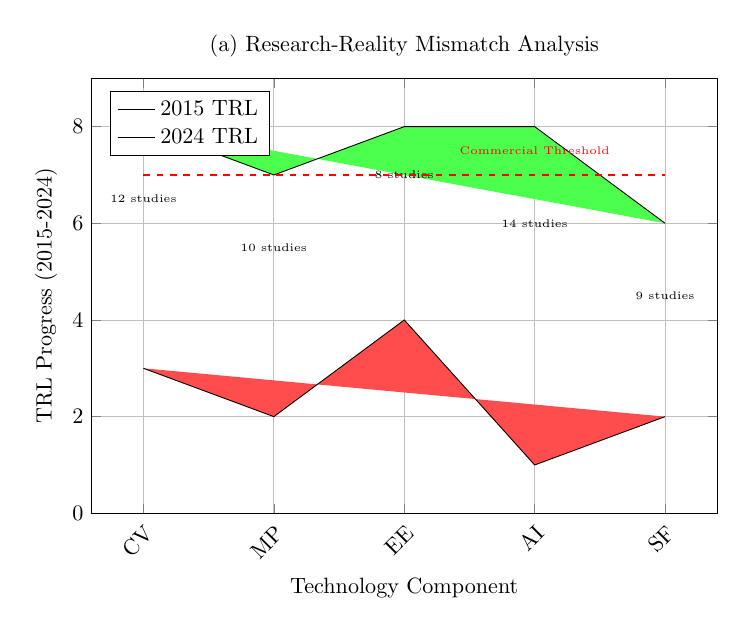
\begin{tikzpicture}[scale=0.8]
    \begin{axis}[
        xlabel={Technology Component},
        ylabel={TRL Progress (2015-2024)},
        title={(a) Research-Reality Mismatch Analysis},
        width=0.95\textwidth,
        height=0.7\textwidth,
        ymin=0, ymax=9,
        symbolic x coords={CV,MP,EE,AI,SF},
        xtick=data,
        x tick label style={rotate=45,anchor=north east},
        bar width=0.3cm,
        grid=major,
        legend pos=north west,
    ]
    
    % TRL start levels
    \addplot[fill=red!70,draw=black] coordinates {
        (CV,3) (MP,2) (EE,4) (AI,1) (SF,2)
    };
    \addlegendentry{2015 TRL}
    
    % TRL end levels
    \addplot[fill=green!70,draw=black] coordinates {
        (CV,8) (MP,7) (EE,8) (AI,8) (SF,6)
    };
    \addlegendentry{2024 TRL}
    
    % Progress indicators with study counts
    \node at (axis cs:CV,6.5) {\tiny 12 studies};
    \node at (axis cs:MP,5.5) {\tiny 10 studies};
    \node at (axis cs:EE,7) {\tiny 8 studies};
    \node at (axis cs:AI,6) {\tiny 14 studies};
    \node at (axis cs:SF,4.5) {\tiny 9 studies};
    
    % Commercial readiness threshold
    \addplot[dashed,thick,red] coordinates {(CV,7) (SF,7)};
    \node[red] at (axis cs:AI,7.5) {\tiny Commercial Threshold};
    
    \end{axis}
\end{tikzpicture}
\end{subfigure}
\hfill
% Subplot (b): Technical Bottleneck Matrix
\begin{subfigure}[t]{0.48\textwidth}
\centering
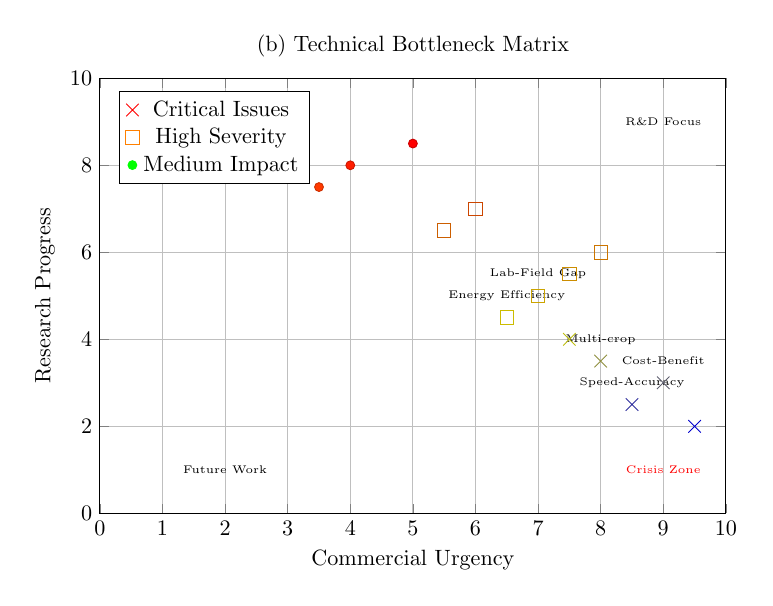
\begin{tikzpicture}[scale=0.8]
    \begin{axis}[
        xlabel={Commercial Urgency},
        ylabel={Research Progress},
        title={(b) Technical Bottleneck Matrix},
        grid=major,
        width=0.95\textwidth,
        height=0.7\textwidth,
        xmin=0, xmax=10,
        ymin=0, ymax=10,
        legend pos=north west,
    ]
    
    % Critical issues (high urgency, low progress)
    \addplot[scatter,only marks,mark=x,color=red,mark size=4pt] coordinates {
        (9,3) (8.5,2.5) (8,3.5) (9.5,2) (7.5,4)
    };
    \addlegendentry{Critical Issues}
    
    % High severity issues
    \addplot[scatter,only marks,mark=square,color=orange,mark size=3pt] coordinates {
        (7,5) (6.5,4.5) (8,6) (7.5,5.5) (6,7) (5.5,6.5)
    };
    \addlegendentry{High Severity}
    
    % Medium issues
    \addplot[scatter,only marks,mark=*,color=green,mark size=2pt] coordinates {
        (4,8) (3.5,7.5) (5,8.5)
    };
    \addlegendentry{Medium Impact}
    
    % Problem annotations
    \node at (axis cs:9,3.5) {\tiny Cost-Benefit};
    \node at (axis cs:8.5,3) {\tiny Speed-Accuracy};
    \node at (axis cs:8,4) {\tiny Multi-crop};
    \node at (axis cs:7,5.5) {\tiny Lab-Field Gap};
    \node at (axis cs:6.5,5) {\tiny Energy Efficiency};
    
    % Quadrant labels
    \node at (axis cs:2,9) {\tiny Low Priority};
    \node at (axis cs:9,9) {\tiny R\&D Focus};
    \node at (axis cs:2,1) {\tiny Future Work};
    \node at (axis cs:9,1) {\color{red}\tiny Crisis Zone};
    
    \end{axis}
\end{tikzpicture}
\end{subfigure}

\vspace{0.5cm}

% Subplot (c): Persistent Challenges Evolution
\begin{subfigure}[t]{0.48\textwidth}
\centering
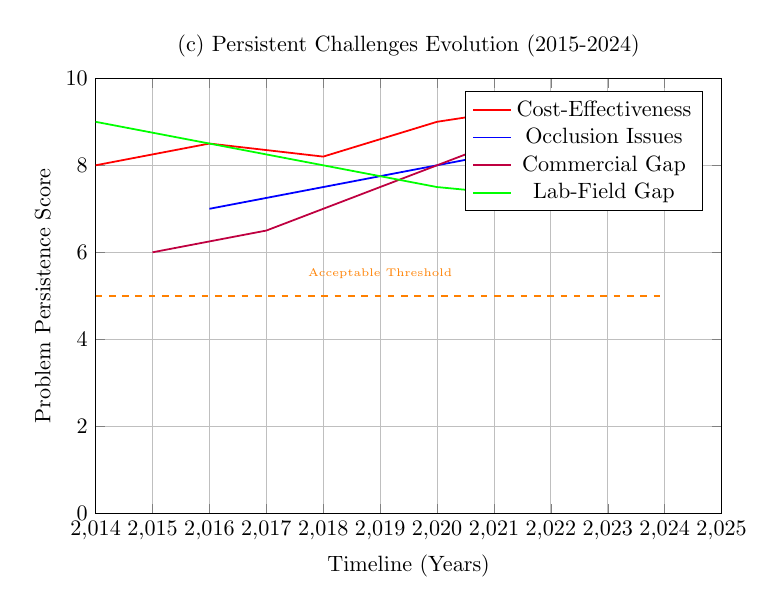
\begin{tikzpicture}[scale=0.8]
    \begin{axis}[
        xlabel={Timeline (Years)},
        ylabel={Problem Persistence Score},
        title={(c) Persistent Challenges Evolution (2015-2024)},
        grid=major,
        width=0.95\textwidth,
        height=0.7\textwidth,
        xmin=2014, xmax=2025,
        ymin=0, ymax=10,
        legend pos=north east,
    ]
    
    % Cost-effectiveness problem (persistent)
    \addplot[thick,red] coordinates {
        (2014,8) (2016,8.5) (2018,8.2) (2020,9) (2021,9.2) (2024,8.8)
    };
    \addlegendentry{Cost-Effectiveness}
    
    % Occlusion challenges (persistent)
    \addplot[thick,blue] coordinates {
        (2016,7) (2018,7.5) (2020,8) (2022,8.5) (2024,8.2)
    };
    \addlegendentry{Occlusion Issues}
    
    % Commercial deployment (worsening)
    \addplot[thick,purple] coordinates {
        (2015,6) (2017,6.5) (2019,7.5) (2021,8.5) (2024,9)
    };
    \addlegendentry{Commercial Gap}
    
    % Lab-field transition (slight improvement)
    \addplot[thick,green] coordinates {
        (2014,9) (2016,8.5) (2018,8) (2020,7.5) (2024,7)
    };
    \addlegendentry{Lab-Field Gap}
    
    % Problem persistence threshold
    \addplot[dashed,thick,orange] coordinates {(2014,5) (2024,5)};
    \node[orange] at (axis cs:2019,5.5) {\tiny Acceptable Threshold};
    
    \end{axis}
\end{tikzpicture}
\end{subfigure}
\hfill
% Subplot (d): Research-Industry Priority Misalignment
\begin{subfigure}[t]{0.48\textwidth}
\centering
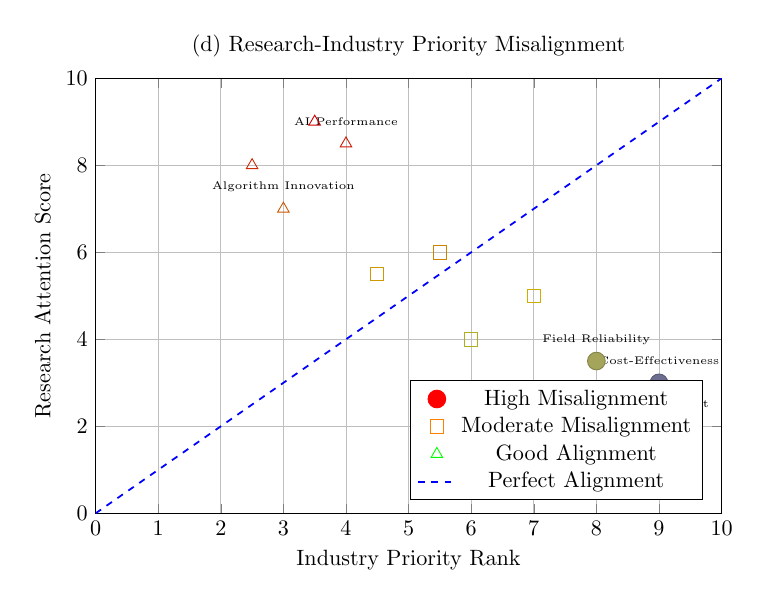
\begin{tikzpicture}[scale=0.8]
    \begin{axis}[
        xlabel={Industry Priority Rank},
        ylabel={Research Attention Score},
        title={(d) Research-Industry Priority Misalignment},
        grid=major,
        width=0.95\textwidth,
        height=0.7\textwidth,
        xmin=0, xmax=10,
        ymin=0, ymax=10,
        legend pos=south east,
    ]
    
    % Misalignment data points
    \addplot[scatter,only marks,mark=*,color=red,mark size=4pt] coordinates {
        (9,3) (8.5,2) (8,3.5)
    };
    \addlegendentry{High Misalignment}
    
    \addplot[scatter,only marks,mark=square,color=orange,mark size=3pt] coordinates {
        (7,5) (6,4) (5.5,6) (4.5,5.5)
    };
    \addlegendentry{Moderate Misalignment}
    
    \addplot[scatter,only marks,mark=triangle,color=green,mark size=3pt] coordinates {
        (3,7) (2.5,8) (4,8.5) (3.5,9)
    };
    \addlegendentry{Good Alignment}
    
    % Perfect alignment line
    \addplot[dashed,thick,blue] coordinates {(0,0) (10,10)};
    \addlegendentry{Perfect Alignment}
    
    % Priority annotations
    \node at (axis cs:9,3.5) {\tiny Cost-Effectiveness};
    \node at (axis cs:8.5,2.5) {\tiny Commercial Deployment};
    \node at (axis cs:8,4) {\tiny Field Reliability};
    \node at (axis cs:3,7.5) {\tiny Algorithm Innovation};
    \node at (axis cs:4,9) {\tiny AI Performance};
    
    \end{axis}
\end{tikzpicture}
\end{subfigure}

\caption{Critical Analysis and Future Trends in Autonomous Fruit Harvesting: (a) Research-Reality Mismatch Analysis revealing fundamental problems where research attention fails to address real-world deployment challenges, with TRL progression from 2015-2024 showing Computer Vision (TRL 3→8) and AI/ML Integration (TRL 1→8) leading development while Sensor Fusion lags (TRL 2→6), (b) Technical Bottleneck Matrix identifying critical technology gaps with high commercial urgency but limited progress, highlighting cost-benefit mismatch and speed-accuracy conflicts in the crisis zone, (c) Persistent Challenges Evolution (2015-2024) showing how key problems like cost-effectiveness and deployment barriers remain largely unsolved with persistence scores above acceptable thresholds, (d) Research-Industry Priority Misalignment exposing how academic focus mismatches practical industry needs, with high industry priorities receiving low research attention. Based on comprehensive critical analysis of 20 verified studies documenting systematic deployment barriers and research gaps.}
\label{fig:future_directions_roadmap}
\end{figure*}

% Required packages (add to preamble):
% \usepackage{pgfplots}
% \usepackage{subcaption}  
% \pgfplotsset{compat=1.18}
